\chapter{无人机网络的能量均衡路由与功率控制}
\label{rq1:chapter}

\section{引言}

在地震、山体滑坡等突发灾害发生后，固定基站和有线传输设施可能同时受损，现场信息难以及时回传。无人机具备快速部署和灵活移动的特点，可以在灾区上空形成临时飞行自组网，为地面传感设备、救援人员和指挥中心提供数据转发服务。在这一过程中，无人机既是信息采集节点，也是其他节点的中继。某一架无人机的通信能力下降，影响的不仅是其自身数据，还可能波及经由该节点转发的多条数据流。因此，通信服务能否持续运行，需要从网络整体状态出发进行分析\cite{intro3,intro4}。

高动态飞行自组网的路由选择同时受到拓扑和能量两方面约束。一方面，节点位置持续变化，原本具有较高传输速率的链路可能在短时间内变弱甚至中断，依赖全局拓扑收集和多轮路径搜索的方法难以及时响应。另一方面，承担大量转发任务的中继节点消耗能量更快，若后续路由仍然优先选择这些节点，就会形成持续加重的能量热点。当热点节点退出网络后，其他节点需要绕行，更多数据将进入缓冲区，部分数据还会因队列溢出而丢失。瞬时看来较短的路径，未必能够在整个任务周期内提供较好的服务。

图\ref{rq1:fig:scenario}给出了典型路由选择场景。发送节点可以通过多个邻居接近数据中心，其中距离较近的候选节点可能已经承担较多中继业务，剩余能量不足；另一候选节点虽然在地理位置上的优势较小，却具有较好的链路条件和更充足的能量。路由策略需要比较这两种选择对当前发送效率和后续通信能力的影响。与此同时，发射功率也应随节点状态变化：功率过低会造成数据积压，功率过高则可能使有限通信能量过早消耗。下一跳选择与功率控制因而具有紧密联系，不能仅通过独立优化某一个因素获得满意结果。

\begin{figure}[!htbp]
  \centering
  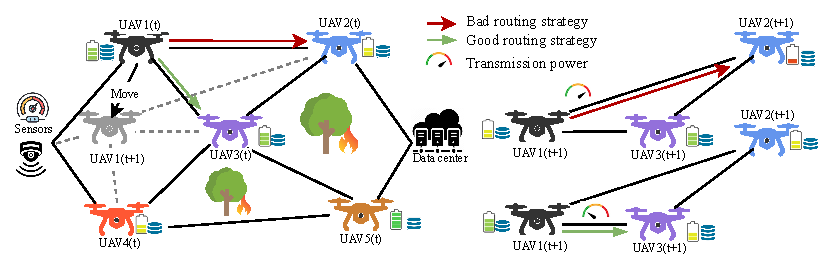
\includegraphics[width=0.96\textwidth]{figures/rq1/scenario.pdf}
  \bicaption{无人机集群中的多跳通信与能量感知路由场景}{Multi-hop communication and energy-aware routing in a UAV swarm}
  \label{rq1:fig:scenario}
\end{figure}

已有地理路由方法利用节点位置实现轻量决策，适合拓扑变化较快的环境，但其转发偏好容易集中在靠近目的节点的少数中继上\cite{gpsr}。负载均衡机制能够分散转发次数，却不一定使实际能耗均衡，因为不同链路完成相同数据传输所需的功率并不相同。强化学习方法可以学习链路状态与长期回报之间的关系\cite{qtar,drlfr,drlrr}，但在任务周期明确、可用能量有限的场景中，仍需要把能量消耗与持续服务目标直接联系起来。对于计算能力受限的机载设备，还应控制在线决策所需的信息规模与计算开销。

针对上述问题，本章提出基于李雅普诺夫优化的能量感知分布式路由策略 LEADR。该策略以全网转发能力为优化目标，通过数据队列、累计能量损耗和虚拟能量队列描述节点的短期压力与长期资源状态，将跨时隙问题转化为逐时隙局部决策。在每个时隙内，节点先计算候选链路的发射功率，再结合下一跳剩余能量和地理进度选择中继。整个过程仅依赖本地状态及邻居广播，不要求获得全网未来运动轨迹。

本章首先建立网络、通信和能量模型，给出任务周期内的联合优化问题；随后推导李雅普诺夫漂移上界，说明虚拟能量队列与累计预算的关系，并给出闭式功率控制和分布式路由流程；最后从无人机数量、通信范围和飞行速度三个方面开展实验分析。该研究为后续语义通信提供基础传输能力，重点解决有限通信能量应如何在节点和时隙之间分配的问题。

\section{系统模型与问题描述}
\label{rq1:sec:model}

\subsection{网络结构与节点移动}

考虑由 $N$ 架无人机和一个数据中心构成的通信网络，无人机集合记为 $\mathcal{N}=\{1,2,\ldots,N\}$，数据中心记为 $D$。无人机负责收集地面数据并通过多跳转发将其送达数据中心。任务持续时间为 $T$，划分为 $K$ 个等长时隙，满足 $T=K\Delta t$，其中 $\Delta t$ 为决策间隔，时隙编号为 $t=0,1,\ldots,K-1$。采用时隙模型有助于在同一时间尺度内描述链路评估、路由选择、数据发送与能量更新。

所有无人机保持固定飞行高度，因此其平面位置和速度分别表示为 $\bm q_i(t)\in\mathbb{R}^{2}$ 与 $\bm v_i(t)\in\mathbb{R}^{2}$。对于任意两个节点，有
\begin{equation}
 d_{ij}(t)=\|\bm q_i(t)-\bm q_j(t)\|_2.
 \label{rq1:eq:distance}
\end{equation}
给定通信范围 $R$，节点 $i$ 的当前邻居集合为
\begin{equation}
 \mathcal{N}_i(t)=\{j\in\mathcal{N}\setminus\{i\}:d_{ij}(t)\le R,\ E_j(t)>0\}.
 \label{rq1:eq:neighbors}
\end{equation}
若数据中心位于通信范围内，则将其加入候选接收节点集合。数据中心不受无人机通信能量预算限制，且不再将已接收的数据作为普通中继数据继续转发。

实验采用高斯--马尔可夫移动模型产生连续相关的运动过程。与每个时隙独立重采样位置相比，该模型能够保留相邻时隙之间的运动惯性，使邻居关系既具有一定持续性，也随速度变化产生更新。路由算法不改变飞行任务，只依据已经发生的移动更新通信决策。这一区分使问题集中于路由层可控制的变量，避免将飞行轨迹优化和通信策略优化混为同一问题。

各节点通过 HELLO 消息交换局部状态。消息包含节点标识、时间戳、位置、速度、剩余能量、数据队列长度及虚拟能量队列长度。接收方据此维护带时间戳的邻居表，并在状态过期或链路预测失效时移除相应记录。邻居表用于决策，不意味着节点已经获得网络全局状态。主要符号如表\ref{rq1:tab:notation}所示。

\begin{table}[!htbp]
\centering\small
\bicaption{能量均衡路由模型的主要符号}{Main notation of the energy-balanced routing model}
\label{rq1:tab:notation}
\begin{tabularx}{\textwidth}{lX}
\toprule
符号 & 含义 \\
\midrule
$\mathcal{N},\mathcal{N}_i(t)$ & 无人机集合及节点 $i$ 在时隙 $t$ 的邻居集合 \\
$T,K,\Delta t$ & 任务持续时间、时隙数与决策间隔 \\
$\bm q_i(t),\bm v_i(t)$ & 节点位置与速度向量 \\
$d_{ij}(t),R$ & 节点间距离与通信范围 \\
$x_{ij}(t),p_{ij}(t)$ & 下一跳选择指示量与链路发射功率 \\
$h_{ij}(t),I_{ij}(t)$ & 链路增益与接收端并发干扰 \\
$r_{ij}(t),\mu_i(t),\nu_i(t)$ & 链路速率、节点服务速率与数据到达速率 \\
$Q_i(t),Q_{\max}$ & 数据积压与缓存容量上限 \\
$E_i(t),E_{\max}$ & 剩余通信能量与初始通信能量预算 \\
$\Phi_i(t),F_i(t)$ & 累计能量损耗与虚拟能量队列 \\
$\beta,\gamma,V$ & 能量损耗、预算偏差与吞吐收益的控制权重 \\
$W_{ij}(t),W_{ij}^{E,G}(t)$ & 基础链路权重与能量、地理修正后的链路权重 \\
\bottomrule
\end{tabularx}
\end{table}

\subsection{链路速率与并发干扰}

无人机之间以视距链路为主，采用自由空间路径损耗模型\cite{qtar}。链路 $(i,j)$ 的信道功率增益表示为
\begin{equation}
 h_{ij}(t)=\frac{\rho_0}{d_{ij}^{2}(t)},\qquad
 \rho_0=\frac{G_iG_j\lambda_c^{2}}{(4\pi)^2},
 \label{rq1:eq:gain}
\end{equation}
其中 $G_i$ 和 $G_j$ 为天线增益，$\lambda_c$ 为载波波长，$\rho_0$ 为参考距离对应的增益参数。该模型主要描述节点间距离对通信条件的影响，未将建筑物遮挡造成的非视距衰落纳入本章优化变量。

令 $x_{ij}(t)\in\{0,1\}$ 表示节点 $i$ 是否选择节点 $j$ 作为下一跳，$p_{ij}(t)$ 表示相应发射功率。同一时隙内，每架无人机至多向一个节点发送数据。考虑其他并发发送节点在接收端形成的干扰，链路信干噪比为
\begin{align}
 I_{ij}(t)&=\sum_{k\in\mathcal{N}\setminus\{i\}}\ \sum_{l\ne k}
              x_{kl}(t)h_{kj}(t)p_{kl}(t),
 \label{rq1:eq:interference}\\
 \operatorname{SINR}_{ij}(t)&=\frac{h_{ij}(t)p_{ij}(t)}{I_{ij}(t)+\sigma^2},
 \label{rq1:eq:sinr}\\
 r_{ij}(t)&=B\log_2\!\left(1+\operatorname{SINR}_{ij}(t)\right),
 \label{rq1:eq:rate}
\end{align}
其中 $B$ 为带宽，$\sigma^2$ 为噪声功率。数据量与速率采用一致单位；若速率以比特每秒表示，则队列数据量相应换算为比特。

式\eqref{rq1:eq:interference}表明，各节点的功率决策在全局范围内相互耦合。节点 $i$ 提高发射功率，可以提高自身链路的信干噪比，但也可能增大其他接收节点的干扰。为获得低复杂度分布式决策，LEADR 在评估一条候选链路时，将根据当前观测得到的干扰作为给定量。后文的闭式解对应这一局部子问题，其适用条件是候选链路的增益和背景干扰在本次评估中保持固定。

\subsection{数据队列与通信能量}

每个无人机节点维护有限容量数据缓冲区。记 $Q_i(t)$ 为时隙开始时的积压，$\lambda_i(t)$ 为本地产生的数据速率。节点的可用服务速率与总到达速率分别为
\begin{equation}
 \mu_i(t)=\sum_j x_{ij}(t)r_{ij}(t),\qquad
 \nu_i(t)=\lambda_i(t)+\sum_k s_{ki}(t),
 \label{rq1:eq:arrival_service}
\end{equation}
其中 $s_{ki}(t)$ 为链路 $(k,i)$ 实际成功转发的速率。队列充足且链路发送成功时，$s_{ki}(t)$ 等于对应链路服务速率；若发送方数据不足，则实际发送量由其积压限制。采用这一写法能够区分链路提供的发送能力与实际存在的数据量。

先定义不考虑容量截断的时隙末队列
\begin{equation}
 Q_i^{+}(t+1)=[Q_i(t)-\mu_i(t)\Delta t]^++\nu_i(t)\Delta t,
 \label{rq1:eq:queue_uncapped}
\end{equation}
其中 $[z]^+=\max\{z,0\}$。有限缓冲区的状态和溢出量为
\begin{equation}
 Q_i(t+1)=\min\{Q_i^{+}(t+1),Q_{\max}\},\qquad
 L_i^{\mathrm{drop}}(t)=[Q_i^{+}(t+1)-Q_{\max}]^+.
 \label{rq1:eq:queue_capped}
\end{equation}
数据队列将过去的发送不足积累为当前可观测压力。当某节点长时间承担较多业务时，队列增大会提高及时转发的需求；当可用链路较少或传输失败较多时，这种压力同样会逐步积累。有限缓存只能限制积压上限，不能消除拥塞，因此还需结合丢包率判断服务质量。

路由层直接控制的是通信发射能量。飞行轨迹由任务安排确定，推进能耗在本章中视为外部开销，$E_{\max}$ 表示单架无人机可用于通信的预算。节点总发射功率与能量更新为
\begin{align}
 P_i(t)&=\sum_j x_{ij}(t)p_{ij}(t),\qquad e_i(t)=P_i(t)\Delta t,
 \label{rq1:eq:power_total}\\
 E_i(t+1)&=E_i(t)-e_i(t),\qquad E_i(0)=E_{\max}.
 \label{rq1:eq:energy_update}
\end{align}
每次发送应满足 $e_i(t)\le E_i(t)$。当通信能量耗尽时，节点退出通信网络，不再参与接收和转发。本章所分析的生命周期由该通信预算模型决定，不直接对应无人机包括飞行、感知和计算在内的整机续航时间。

即使两架无人机转发相同数量的数据，也可能具有不同的能耗。较远的链路或较强的干扰会改变所需功率，数据积压和发送时机也会影响累计消耗。因此，仅平均分配转发次数并不足以控制剩余能量差异，需要把功率与路由放在同一状态反馈过程中考虑。

\subsection{任务周期内的联合优化问题}

令 $\pi$ 表示根据当前可用状态生成下一跳和功率的因果控制策略。沿用本研究对全网链路转发能力的度量，考虑任务周期内平均聚合服务速率
\begin{equation}
 \overline{U}(\pi)=\frac{1}{K}\sum_{t=0}^{K-1}
                 \sum_{i\in\mathcal{N}}\E_{\pi}[\mu_i(t)].
 \label{rq1:eq:utility}
\end{equation}
该指标统计各节点提供的转发服务，一份数据经由多个中继时会占用多条链路。因此，聚合服务速率体现网络转发资源的利用程度，与数据中心收到的去重业务数据量具有不同含义。实验同时报告丢包率和生命周期，以避免仅依据链路活动量判断服务效果。

将发射功率、转发对象、缓存容量和可用通信预算写入约束，可得
\begin{align}
 \max_{\pi}\quad &\overline{U}(\pi),\label{rq1:eq:problem}\\
 \text{s.t.}\quad
 &0\le p_{ij}(t)\le P_{\max},\quad x_{ij}(t)\in\{0,1\},\nonumber\\
 &\sum_jx_{ij}(t)\le1,\quad x_{ij}(t)=0\ \text{若链路 $(i,j)$ 不可用},\nonumber\\
 &0\le Q_i(t)\le Q_{\max},\quad 0\le e_i(t)\le E_i(t),\nonumber\\
 &\sum_{t=0}^{K-1}e_i(t)\le E_{\max},\qquad \forall i\in\mathcal{N}.\nonumber
\end{align}
其中，队列容量通过实际缓存操作实现，能量约束通过当前可用能量限制发送行为。约束满足并不自动意味着较低丢包或较长服务时间，策略仍可能过早用尽预算，或因过于保守而使数据滞留。因此，需要在满足物理边界的同时调整能量消耗节奏。

直接求解式\eqref{rq1:eq:problem}需要考虑当前动作对未来拓扑、队列和节点存活状态的影响，而这些信息在动态任务中难以提前获得。此外，离散路由变量与连续功率变量共同决定链路速率，节点间又通过干扰耦合。LEADR 采用逐时隙优化框架形成局部决策依据，再利用地理进度和下一跳能量信息修正路由选择，以控制在线求解规模。

\section{基于李雅普诺夫漂移的能量控制}
\label{rq1:sec:lyapunov}

\subsection{虚拟能量队列与预算偏差}

为了描述节点相对于任务时间进度的能量消耗，引入可持续平均功率和平均时隙能量预算
\begin{equation}
 P_{\mathrm{avg}}=\frac{E_{\max}}{T},\qquad
 \bar e=P_{\mathrm{avg}}\Delta t=\frac{E_{\max}}{K}.
 \label{rq1:eq:average_budget}
\end{equation}
这里的平均预算不是每个时隙必须严格执行的固定额度。突发数据到来时，允许节点短时间内超过平均水平；在负载较轻或链路不利时，则可以降低发送功率。为了在后续决策中保留这种超额消耗的信息，定义虚拟能量队列
\begin{equation}
 F_i(t+1)=[F_i(t)+e_i(t)-\bar e]^+,\qquad F_i(0)=0.
 \label{rq1:eq:virtual_queue}
\end{equation}
当本时隙能耗高于平均预算时，$F_i(t)$ 增大；低于平均预算时，队列逐步回落，最低为零。该状态记录的是尚未消化的预算偏差，不是实际剩余电量。因此，两个当前剩余能量接近的节点，如果过去一段时间的负载不同，其虚拟队列也可能不同。

\begin{proposition}[虚拟队列的累计预算关系]
\label{rq1:prop:budget}
对于按式\eqref{rq1:eq:virtual_queue}更新的虚拟能量队列，任意 $1\le m\le K$ 均满足
\begin{equation}
 \sum_{t=0}^{m-1}e_i(t)\le m\bar e+F_i(m)-F_i(0).
 \label{rq1:eq:finite_budget}
\end{equation}
\end{proposition}
\begin{proof}
由 $[z]^+\ge z$，有 $F_i(t+1)-F_i(t)\ge e_i(t)-\bar e$。对 $t=0,\ldots,m-1$ 求和，左侧相邻项相消，即可得到式\eqref{rq1:eq:finite_budget}。
\end{proof}

该关系说明，虚拟队列上升意味着累计能耗可能偏离均匀预算轨迹，抑制队列增长有助于控制这种偏离。若考虑无限时域并额外满足均值速率稳定条件 $\E[F_i(m)]/m\to0$，还可以得到平均能耗不超过 $\bar e$ 的结论。对于本章的有限任务，式\eqref{rq1:eq:finite_budget}保留了终端偏差项 $F_i(K)$，因此真实能量可行性仍需由式\eqref{rq1:eq:energy_update}及可用能量约束保证。虚拟队列承担的是引导消耗节奏的作用。

\subsection{李雅普诺夫函数与漂移上界}

除虚拟能量队列外，定义累计通信能量损耗
\begin{equation}
 \Phi_i(t)=E_{\max}-E_i(t),\qquad
 \Phi_i(t+1)=\Phi_i(t)+e_i(t).
 \label{rq1:eq:energy_deficit}
\end{equation}
$\Phi_i(t)$ 随实际消耗累积，用于表示节点已经使用的通信资源。其与 $F_i(t)$ 的区别在于，前者反映任务开始至今的总消耗，后者反映相对于平均预算的偏差。二者共同作用，可以使早期消耗较多、近期又持续超额的节点承担更高的能量代价。

根据队列控制方法\cite{algo1,algo2,intro13}，定义节点李雅普诺夫函数
\begin{equation}
 L_i(t)=\frac{1}{2}Q_i^2(t)+\frac{\beta}{2}\Phi_i^2(t)
                 +\frac{\gamma}{2}F_i^2(t),
 \label{rq1:eq:lyapunov}
\end{equation}
其中 $\beta,\gamma\ge0$ 为权重，吸收不同状态的量纲和尺度差异。$L_i(t)$ 是当前积压与资源压力的度量。由于通信能量不会在任务中补充，累计损耗 $\Phi_i(t)$ 不会像数据队列一样通过服务而减小，因此这里不要求其收敛到零。

令 $\Theta(t)$ 表示时隙 $t$ 已观测到的队列、能量和链路状态，单步条件漂移为
\begin{equation}
 \Delta_i(t)=\E[L_i(t+1)-L_i(t)\mid\Theta(t)].
 \label{rq1:eq:drift}
\end{equation}
漂移刻画执行一次控制动作后状态压力的预期变化。为了同时鼓励有效转发，在漂移中减去 $V$ 加权的服务收益，得到漂移减收益形式 $\Delta_i(t)-V\E[\mu_i(t)\mid\Theta(t)]$，其中 $V\ge0$。

下面分别处理三个状态的平方项。对于数据队列，利用 $([Q-b]^++a)^2\le Q^2+a^2+b^2+2Q(a-b)$，有
\begin{equation}
 \frac{Q_i^2(t+1)-Q_i^2(t)}{2}
 \le\frac{\Delta t^2}{2}\bigl[\nu_i^2(t)+\mu_i^2(t)\bigr]
       +Q_i(t)\Delta t[\nu_i(t)-\mu_i(t)].
 \label{rq1:eq:queue_drift}
\end{equation}
有限缓存的截断只会减小下一时隙队列，因此不改变该上界的有效性。对于累计能量损耗，由式\eqref{rq1:eq:energy_deficit}直接展开可得
\begin{equation}
 \frac{\beta}{2}[\Phi_i^2(t+1)-\Phi_i^2(t)]
 =\beta\Phi_i(t)e_i(t)+\frac{\beta}{2}e_i^2(t).
 \label{rq1:eq:energy_drift}
\end{equation}
虚拟能量队列满足 $([F+e-\bar e]^+)^2\le(F+e-\bar e)^2$，因而
\begin{equation}
 \frac{\gamma}{2}[F_i^2(t+1)-F_i^2(t)]
 \le\gamma F_i(t)[e_i(t)-\bar e]
       +\frac{\gamma}{2}[e_i(t)-\bar e]^2.
 \label{rq1:eq:virtual_drift}
\end{equation}

若数据到达和服务速率的条件二阶矩有界，且发射功率满足上限，则三个式子中的二次增量项可由有限常数 $C$ 统一上界。泊松到达过程具有有限二阶矩，这一条件不要求每个时隙的数据到达量完全相同。对上述关系取条件期望并相加，有
\begin{align}
 &\Delta_i(t)-V\E[\mu_i(t)\mid\Theta(t)]\nonumber\\
 &\quad\le C+\E\bigl[Q_i(t)\Delta t\nu_i(t)
       -(Q_i(t)\Delta t+V)\mu_i(t)\nonumber\\
 &\hspace{42mm}
       +(\beta\Phi_i(t)+\gamma F_i(t))e_i(t)
       -\gamma F_i(t)\bar e\mid\Theta(t)\bigr].
 \label{rq1:eq:dpp_bound}
\end{align}
该上界把跨时隙状态的影响转化为当前队列和能量权重，使节点无需知道未来到达量和移动轨迹，即可比较本时隙动作的收益与代价。

\subsection{局部决策目标及能量均衡作用}

为简化表达，定义
\begin{equation}
 C_i(t)=\beta\Phi_i(t)+\gamma F_i(t),\qquad
 D_i(t)=Q_i(t)\Delta t+V.
 \label{rq1:eq:coefficients}
\end{equation}
去掉与当前控制无关的常数项后，节点需要降低的局部目标为
\begin{equation}
 Q_i(t)\Delta t\nu_i(t)-D_i(t)\mu_i(t)+C_i(t)\Delta tP_i(t).
 \label{rq1:eq:local_objective}
\end{equation}
在评估节点自身的下一跳与功率时，到达项根据当前邻居活动作为给定量处理。由于一个节点的发送也会影响接收节点的积压和其他链路干扰，这一步属于分布式局部近似。若要求联合最小化全网漂移，需要同时考虑发送端和接收端的队列差以及所有功率的耦合，求解规模将随网络扩大而增长。LEADR 保留可在本地计算的权重，并通过后续启发式选择补充空间转发约束。

$D_i(t)$ 表示发送收益权重。队列增大时，同样的服务速率能够缓解更多积压压力，节点倾向于及时发送；即使积压较小，$V$ 也保留对转发能力的偏好。$C_i(t)$ 表示能量价格，累计消耗或预算偏差越大，相同功率对应的代价越高。这两个权重随任务运行自动变化，使功率控制能够响应业务和能量状态，而无需对每个节点预先设置固定发送比例。

累计损耗的二次项还具有抑制消耗集中现象的作用。记全网平均损耗为 $\bar\Phi(t)=N^{-1}\sum_i\Phi_i(t)$，则
\begin{equation}
 \sum_i\Phi_i^2(t)=N\bar\Phi^2(t)
                  +\sum_i[\Phi_i(t)-\bar\Phi(t)]^2.
 \label{rq1:eq:energy_variance_identity}
\end{equation}
在总损耗相同的情况下，消耗越集中，右侧第二项越大。因此，引入平方损耗会使持续承担较多转发任务的节点面临更高的边际代价。这为能量均衡提供了明确的数学解释，但并不意味着所有节点应消耗完全相同的能量。不同节点的位置和数据负载具有差异，适度的不均衡可能是提高整体转发效率所必需的。

参数 $\beta$、$\gamma$ 和 $V$ 分别调节累计能耗、消耗节奏与服务收益的相对重要性。增大 $\beta$ 会提高已消耗较多节点继续发送的代价；增大 $\gamma$ 会使短期超额消耗更快受到抑制；增大 $V$ 通常会提高发送积极性，但也会增加能量使用压力。由于实际算法包含干扰近似和路由修正，本章不将经典全局漂移最小化方法的最优性间隙直接作为 LEADR 的保证，而通过明确的局部性质和实验评价其实际效果。

\section{分布式路由与功率联合决策}
\label{rq1:sec:algorithm}

\subsection{候选链路的闭式功率控制}

对给定候选下一跳 $j$，记 $N_{ij}(t)=I_{ij}(t)+\sigma^2>0$。在本次链路评估中固定 $h_{ij}(t)$ 和 $N_{ij}(t)$，将式\eqref{rq1:eq:rate}代入局部目标，得到
\begin{equation}
 \min_{0\le p\le P_{\max}} f_{ij}(p),\qquad
 f_{ij}(p)=-D_i(t)B\log_2\!\left(1+\frac{h_{ij}(t)p}{N_{ij}(t)}\right)
                         +C_i(t)\Delta t\,p.
 \label{rq1:eq:power_problem}
\end{equation}
该子问题在服务速率与线性能耗之间进行权衡，只包含一个连续变量。其一阶与二阶导数分别为
\begin{align}
 f'_{ij}(p)&=-\frac{D_i(t)Bh_{ij}(t)}{\ln2\,[N_{ij}(t)+h_{ij}(t)p]}
                       +C_i(t)\Delta t,
 \label{rq1:eq:first_derivative}\\
 f''_{ij}(p)&=\frac{D_i(t)B h_{ij}^2(t)}{\ln2\,[N_{ij}(t)+h_{ij}(t)p]^2}\ge0.
 \label{rq1:eq:second_derivative}
\end{align}
因此，固定干扰条件下的链路功率目标为凸函数。当 $D_i(t)>0$ 且 $h_{ij}(t)>0$ 时，二阶导数严格为正，区间内的最优解唯一。

\begin{proposition}[固定干扰下的链路功率最优解]
\label{rq1:prop:power}
若 $C_i(t)>0$、$D_i(t)>0$ 且 $h_{ij}(t)>0$，式\eqref{rq1:eq:power_problem}的解为
\begin{equation}
 p_{ij}^{\mathrm{opt}}(t)=
 \left[\frac{D_i(t)B}{\ln2\,C_i(t)\Delta t}
            -\frac{N_{ij}(t)}{h_{ij}(t)}\right]_{0}^{P_{\max}},
 \label{rq1:eq:power_opt}
\end{equation}
其中 $[z]_{a}^{b}=\min\{\max\{z,a\},b\}$ 表示区间截断。
\end{proposition}
\begin{proof}
令式\eqref{rq1:eq:first_derivative}为零，得到无约束驻点。由凸性可知，当驻点位于可行区间内时即为最优点；驻点低于零时，目标在可行区间上递增，最优点为零；驻点高于功率上限时，目标在区间内递减，最优点为上限。三种情况合并即为式\eqref{rq1:eq:power_opt}。
\end{proof}

初始时刻可能出现 $C_i(t)=0$。若此时有待发数据且链路增益为正，目标随功率增加而下降，应选择当前可行的功率上限，无需进行除零计算。若无待发数据、链路不可用或收益权重为零，则不发送。真实可用能量不足以支持一个完整时隙的最大发射功率时，还应将功率上限限制为 $\min\{P_{\max},E_i(t)/\Delta t\}$。这些边界处理与物理约束一致，不改变正常可行区间内的闭式表达。

式\eqref{rq1:eq:power_opt}中，第一项表示由服务需求与能量价格共同确定的发送水平，第二项表示链路的不利程度。较好的信道增益降低了完成传输的资源压力，而累计能耗和虚拟队列增长会降低可接受的功率。高干扰链路并不必然值得提高功率：当边际速率收益不足以抵消能耗时，最优功率会降为零，节点应考虑其他候选下一跳。

\subsection{融合能量状态与地理进度的下一跳选择}

得到候选链路的功率后，计算对应速率 $r_{ij}^{\mathrm{opt}}(t)$，并定义基础权重
\begin{equation}
 W_{ij}(t)=D_i(t)r_{ij}^{\mathrm{opt}}(t)
                   -C_i(t)\Delta t\,p_{ij}^{\mathrm{opt}}(t).
 \label{rq1:eq:base_weight}
\end{equation}
它表示本次链路发送的服务收益扣除能量代价后的净值。由于零功率是可行候选，单链路最优目标不会差于不发送，因此在精确计算和给定干扰的条件下，$W_{ij}(t)\ge0$。实际决策中可将不发送的权重设置为零，使没有正收益候选时保持等待。

基础权重主要反映发送节点的状态，尚未考虑下一跳能否持续承担转发任务。为此，定义候选节点的归一化剩余能量及相对地理进度
\begin{equation}
 \widetilde E_j(t)=\frac{E_j(t)}{E_{\max}},\qquad
 G_{ij}(t)=\frac{d_{iD}(t)-d_{jD}(t)}{d_{iD}(t)}.
 \label{rq1:eq:energy_geography}
\end{equation}
$G_{ij}(t)>0$ 表示下一跳比当前节点更接近数据中心。在满足正地理进度的候选中，归一化剩余能量用于降低低能量中继的优先级，形成复合权重
\begin{equation}
 W_{ij}^{E,G}(t)=
 \begin{cases}
 W_{ij}(t)\widetilde E_j(t),&G_{ij}(t)>0,\ j\ne D,\\
 W_{ij}(t),&j=D\ \text{且链路可用},\\
 -\infty,&\text{其他情况}.
 \end{cases}
 \label{rq1:eq:composite_weight}
\end{equation}
数据中心不再承担后续中继，因此无需乘以无人机能量因子。最终下一跳为
\begin{equation}
 j^*(t)\in\arg\max_jW_{ij}^{E,G}(t).
 \label{rq1:eq:next_hop}
\end{equation}
若所有候选均不可用或净收益为零，则本时隙不发送，保留数据并等待后续状态更新。

该修正采用地理进度作为可行性条件，而不是强制选择进度最大的邻居。只要能够向数据中心推进，就允许链路效率和能量状态决定具体下一跳，因此可以利用多条可行转发方向分担负载。对于某一时刻固定的拓扑快照，沿每一条允许链路到数据中心的距离严格下降，不可能形成距离同时严格下降又返回起点的有向环。由于移动会改变跨时隙的距离关系，这一性质对应当前快照中的转发结构，不等价于任意移动过程下的数据包从不回访历史节点。

正地理进度约束还带来一种取舍。当周围邻居均不比当前节点更接近数据中心时，可能出现暂时转发空洞。LEADR 保留等待动作，利用后续移动带来的新机会，而未在本章中引入额外的周界绕行或全局路径搜索。这保持了低计算复杂度，也意味着稀疏网络中的长时间空洞仍可能造成积压，需要通过实验中的丢包和服务时间观察其影响。

\subsection{基于相对运动的 HELLO 更新机制}

邻居信息的时效性直接影响路由选择。固定广播周期较长时，节点可能继续使用已经离开通信范围的邻居；周期过短时，又会增加控制消息发送和接收开销。参考拓扑感知路由的处理方式\cite{qtar}，LEADR 根据相对运动预测链路剩余寿命，并按其一定比例调整 HELLO 间隔。

以一次状态更新时刻为起点，记 $\bm r_{ij}=\bm q_j-\bm q_i$、$\bm u_{ij}=\bm v_j-\bm v_i$，在短时间内近似保持当前速度，则经过 $\tau$ 后的相对位置为 $\bm r_{ij}+\tau\bm u_{ij}$。链路到达通信边界时满足
\begin{equation}
 \|\bm r_{ij}+\tau\bm u_{ij}\|_2^2=R^2.
 \label{rq1:eq:let_equation}
\end{equation}
令 $a=\|\bm u_{ij}\|_2^2$、$b=\bm r_{ij}^{\mathsf T}\bm u_{ij}$、$c=\|\bm r_{ij}\|_2^2$。对当前范围内的链路，当 $a>0$ 时，其预测离开时间为
\begin{equation}
 \widehat\tau_{ij}=
 \frac{-b+\sqrt{b^2+a(R^2-c)}}{a}.
 \label{rq1:eq:let_solution}
\end{equation}
若相对速度接近零，则在局部线性预测下链路较为稳定；若当前已经超出范围，则相应记录失效。实际飞行轨迹不会始终保持匀速，因此预测用于确定更新频率，而不作为未来连通性的确定性保证。

采用保守邻居预测值时，可将广播间隔写为
\begin{equation}
 \tau_i^{\mathrm{hello}}=
 \operatorname{clip}\!\left(\eta\min_{j\in\mathcal{N}_i}\widehat\tau_{ij},
                          \tau_{\min},\tau_{\max}\right),\qquad 0<\eta<1.
 \label{rq1:eq:hello_interval}
\end{equation}
其中上下限用于避免极短预测造成频繁广播或稳定链路导致长时间不更新，$\eta$ 表示提前更新的比例。邻居表为空时使用周期性发现消息重新获取候选节点。该表达给出了自适应机制的实现形式，实验分析围绕整体路由策略展开，不单独推断 HELLO 参数对收益的独立贡献。

HELLO 消息中的位置和速度用于地理进度及链路寿命估计，剩余能量用于下一跳修正。本地数据队列和虚拟能量队列决定发送端的服务收益与能量价格。各类信息分别作用于拓扑维护、候选筛选和功率求解，使通信决策形成从状态更新到动作执行的完整过程。

\subsection{算法流程与计算复杂度}

算法\ref{rq1:alg:leadr}给出了单节点执行流程。节点在时隙开始时更新邻居信息，然后遍历当前可用候选，对每条链路计算功率、速率和复合权重，选取收益最高的动作。发送结束后，根据实际到达、服务和能量消耗更新三个状态量，作为下一次决策的输入。算法不需要在每次决策前重新训练模型，也不需要迭代搜索完整多跳路径。

\begin{algorithm}[!htbp]
\caption{LEADR 分布式路由与功率联合决策\\\small LEADR decentralized routing and power control}
\label{rq1:alg:leadr}
\small
\begin{algorithmic}[1]
\Require 本地状态 $Q_i(t),E_i(t),F_i(t)$，邻居表，通信与控制参数
\Ensure 下一跳 $j^*(t)$、路由指示量 $x_{ij}(t)$ 与发射功率
\State 依据时间戳和相对运动更新邻居表，移除失效记录
\State 根据式\eqref{rq1:eq:coefficients}计算 $C_i(t)$ 和 $D_i(t)$
\State 初始化所有 $x_{ij}(t)\gets0$，最优收益 $w^*\gets0$，动作设为等待
\If{$Q_i(t)>0$ 且 $E_i(t)>0$}
 \For{每个可用候选 $j\in\mathcal{N}_i(t)\cup\{D\}$}
  \If{$j$ 满足向数据中心推进的条件}
   \State 估计 $h_{ij}(t)$ 和 $N_{ij}(t)$，确定当前能量可行的功率上限
   \State 根据式\eqref{rq1:eq:power_opt}及边界情况计算 $p_{ij}^{\mathrm{opt}}(t)$
   \State 计算 $r_{ij}^{\mathrm{opt}}(t)$ 与 $W_{ij}^{E,G}(t)$
   \If{$W_{ij}^{E,G}(t)>w^*$}
    \State 保存候选 $j$、对应功率及收益，更新 $w^*$
   \EndIf
  \EndIf
 \EndFor
\EndIf
\If{存在正收益候选}
 \State 令 $x_{ij^*}(t)\gets1$，以保存的功率向 $j^*$ 发送待发数据
\Else
 \State 不发送，保留队列并等待后续邻居状态更新
\EndIf
\State 依据实际数据收发与能耗更新 $Q_i(t+1),E_i(t+1),F_i(t+1)$
\State 按链路寿命估计调整下一次 HELLO 广播时间
\end{algorithmic}
\end{algorithm}

记节点 $i$ 的邻居数为 $n_i(t)$。单条候选链路的功率计算只包含常数次四则运算、对数和截断操作，地理判断与能量修正也为常数复杂度。通过一次遍历同时维护最优候选，无需对全部邻居排序，因此单节点单时隙决策复杂度为
\begin{equation}
 \mathcal{C}_{i}^{\mathrm{time}}=O(n_i(t)),\qquad
 \mathcal{C}_{i}^{\mathrm{space}}=O(n_i(t)).
 \label{rq1:eq:complexity}
\end{equation}
空间开销主要来自邻居表，除此之外只需保存当前状态与最优动作。全网分布式执行的总运算量与各节点邻居数之和同阶，而不是要求单一控制器集中处理所有动作组合。

表\ref{rq1:tab:components}概括了不同机制与状态信息之间的关系。虚拟能量队列负责时间维度上的预算节奏，下一跳能量因子负责空间维度上的任务分散，地理条件约束转发方向，HELLO 更新维护局部信息时效。这些机制共同形成路由与功率反馈过程。其中闭式功率求解具有明确的局部最优性质，整体下一跳策略仍属于经过能量和地理信息修正的分布式启发式方法。

\begin{table}[!htbp]
\centering\small
\bicaption{LEADR 各组成机制及其作用}{Components of LEADR and their roles}
\label{rq1:tab:components}
\begin{tabularx}{\textwidth}{p{0.22\textwidth}p{0.28\textwidth}X}
\toprule
组成机制 & 主要依据 & 对决策的作用 \\
\midrule
数据队列反馈 & 当前积压 $Q_i(t)$ & 提高拥塞节点的发送收益权重 \\
累计能耗惩罚 & 已用能量 $\Phi_i(t)$ & 降低能量消耗集中节点的持续发送强度 \\
虚拟能量队列 & 实际能耗与平均预算偏差 & 抑制连续超额使用通信能量 \\
闭式功率控制 & 链路增益、干扰与能量价格 & 以常数计算量平衡发送速率和能耗 \\
下一跳能量修正 & 邻居归一化剩余能量 & 降低低能量中继的转发优先级 \\
地理进度限制 & 到数据中心的相对距离 & 限制当前转发方向，减少无效绕行 \\
自适应 HELLO & 邻居相对位置和速度 & 根据拓扑变化调整状态更新频率 \\
\bottomrule
\end{tabularx}
\end{table}

\section{实验设置与结果分析}
\label{rq1:sec:experiments}

\subsection{仿真环境与评价指标}

实验使用 Python 离散事件仿真器，对无人机移动、数据产生、链路传输、缓冲区更新和节点能量消耗进行模拟。仿真区域为 $1000\,\mathrm{m}\times1000\,\mathrm{m}$，单次任务持续 $3600\,\mathrm{s}$，决策间隔为 $1\,\mathrm{s}$。地面数据源按泊松过程产生数据，无人机按照高斯--马尔可夫模型移动。主要物理与通信参数参考已有 FANET 路由研究\cite{qtar,drlfr}，具体设置如表\ref{rq1:tab:settings}所示。三组实验分别改变节点数量、通信范围和平均飞行速度，其余因素在对应实验组内保持一致。

\begin{table}[!htbp]
\centering\small
\bicaption{无人机路由仿真的主要参数}{Main parameters of the UAV routing simulation}
\label{rq1:tab:settings}
\begin{tabularx}{\textwidth}{lX}
\toprule
参数 & 设置 \\
\midrule
仿真区域 & $1000\,\mathrm{m}\times1000\,\mathrm{m}$ \\
任务持续时间、决策间隔 & $3600\,\mathrm{s}$、$1\,\mathrm{s}$ \\
移动模型、业务到达模型 & 高斯--马尔可夫移动、泊松数据到达 \\
信道带宽 $B$ & $20\,\mathrm{MHz}$ \\
噪声功率 $\sigma^2$ & $0.8\times10^{-12}\,\mathrm{W}$ \\
参考信道参数 $\rho_0$ & $10^{-4}$ \\
最大发射功率 $P_{\max}$ & $0.2\,\mathrm{W}$ \\
数据包大小、缓冲区容量 & $1\,\mathrm{KB}$、$8000\,\mathrm{KB}$ \\
单节点通信能量预算 $E_{\max}$ & $15\,\mathrm{J}$ \\
无人机数量实验 & $10,20,30,40,50$ 架 \\
通信范围实验 & $200,225,250,275,300\,\mathrm{m}$，无人机数量为 30 架 \\
平均飞行速度实验 & $5,10,15,20,25\,\mathrm{m/s}$ \\
\bottomrule
\end{tabularx}
\end{table}

对比方法包括四类代表性策略。GPSR 根据地理信息优先选择靠近目的节点的邻居\cite{gpsr}；LB-GPSR 在正地理进度候选之间轮询转发，以分散局部负载；ACO 以蚁群路由中的信息素更新思想为基础\cite{aco}，在本章实现中结合节点能量和距离进行路径选择；RLFR 采用强化学习思想，根据数据投递和通信能耗形成回报，引导路由与功率决策\cite{drlfr}。这些方法分别代表地理贪心、轮询均衡、启发式搜索和学习控制思路。本章比较对应统一仿真环境中的实现，不将某个基线在本场景下的表现推广为其全部应用条件下的性能。

评价围绕以下四个指标展开。网络聚合吞吐量反映全网成功转发数据所形成的平均速率，图中单位为 Mbps；数据包丢失率反映数据因拥塞、不可达和节点退出等原因未能完成传输的比例，数值越低越好；能量均衡指标统计归一化剩余能量的离散程度，数值越低表示节点间差异越小；网络生命周期定义为出现首个通信能量耗尽节点之前的时间。四项指标分别从服务量、业务损失、资源分布和持续时间评价通信效果，能够反映不同路由策略的综合取舍。

对于生命周期，实验统计值为
\begin{equation}
 T_{\mathrm{life}}^{\mathrm{obs}}=
 \min\!\left\{T,\ \inf\{t\Delta t:\exists i,\ E_i(t)\le0\}\right\}.
 \label{rq1:eq:observed_lifetime}
\end{equation}
当一条结果达到 $3600\,\mathrm{s}$ 时，表示在整个观察窗口内未出现由通信能量耗尽引起的首个节点退出，不能据此推断任务结束后的剩余寿命。能量均衡也应与吞吐和丢包联合理解：通信活动较少可能保留较均匀的能量，但这种均匀本身并不能说明通信服务更好。

\subsection{无人机数量变化下的性能分析}
\label{rq1:sec:experiment_size}

第一组实验将无人机数量由 10 架增加至 50 架。节点数量增加同时带来更多候选中继、更多数据转发需求以及更强的并发竞争，因此可以检验算法能否把新增节点转化为有效通信能力。图\ref{rq1:fig:size}给出了五个规模条件下的四项指标。

\begin{figure}[!htbp]
\centering
\begin{subfigure}{0.49\textwidth}\centering
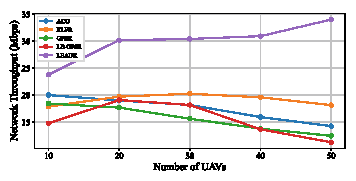
\includegraphics[width=\linewidth]{figures/rq1/num_a.pdf}
\caption{网络聚合吞吐量}\label{rq1:fig:size_a}
\end{subfigure}\hfill
\begin{subfigure}{0.49\textwidth}\centering
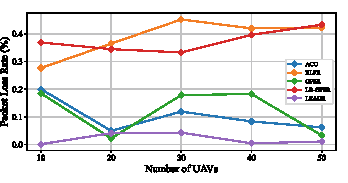
\includegraphics[width=\linewidth]{figures/rq1/num_b.pdf}
\caption{数据包丢失率}\label{rq1:fig:size_b}
\end{subfigure}
\par\medskip
\begin{subfigure}{0.49\textwidth}\centering
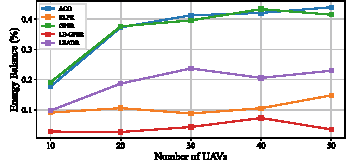
\includegraphics[width=\linewidth]{figures/rq1/num_c.pdf}
\caption{能量均衡指标}\label{rq1:fig:size_c}
\end{subfigure}\hfill
\begin{subfigure}{0.49\textwidth}\centering
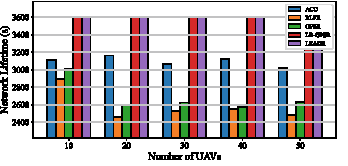
\includegraphics[width=\linewidth]{figures/rq1/num_d.pdf}
\caption{网络生命周期}\label{rq1:fig:size_d}
\end{subfigure}
\bicaption{不同无人机数量下的路由性能比较}{Routing performance with different numbers of UAVs}
\label{rq1:fig:size}
\end{figure}

从图\ref{rq1:fig:size_a}可见，LEADR 的吞吐量总体随规模增加而上升。10 架节点时，其曲线已经高于对比策略；增加到 20 架后，吞吐水平进一步提高；在 30 架和 40 架条件下保持较高水平，50 架条件下继续增长。与之相比，GPSR 和 ACO 随节点数增加总体下降，LB-GPSR 在小规模阶段短暂提高后回落，RLFR 则在中等规模附近相对平缓，随后有所下降。因此，更准确的结论是各基线的规模收益有限，不能仅凭节点增加获得持续的转发能力增长。

这种变化与决策依据有关。地理贪心容易反复使用朝向数据中心的少数位置优势节点，即使网络中加入更多中继，也未必能够均匀利用。轮询可以使更多候选参与，但不同候选的链路质量和发送代价不一致，轮询次数均等不代表有效服务量均等。LEADR 在每个节点内部通过队列压力与能量价格调整功率，在节点之间通过能量权重分散转发，因此更有机会利用密集网络中的替代链路。

图\ref{rq1:fig:size_b}进一步显示，LEADR 在各节点规模下保持较低丢包率，曲线接近横轴。其余策略的表现并非随规模单调变化：例如 ACO 和 GPSR 在部分中等规模条件下丢包下降，随后又随负载与拓扑关系变化而波动。LB-GPSR 和 RLFR 的丢包率整体处于较高区间。较高的聚合吞吐若主要来自重复绕行或无效链路活动，通常难以同时获得较低丢包；本组结果中二者结合，说明 LEADR 增加的转发能力确实有助于维持业务传输。

能量均衡结果需要结合其他指标分析。图\ref{rq1:fig:size_c}中，LEADR 的离散程度明显低于 ACO 和 GPSR，但高于 LB-GPSR 与 RLFR，并未在该指标上取得全方法最小值。随着规模增大，其曲线也存在上升和波动。这表明 LEADR 为了维持较高服务量，允许承担不同任务的节点消耗不同能量，而不是把所有节点的剩余能量强制拉到同一水平。LB-GPSR 较低的离散度具有合理性，但其丢包和吞吐结果说明，仅追求负载平均仍不足以获得较好的综合服务。

从图\ref{rq1:fig:size_d}可见，LEADR 和 LB-GPSR 在本组全部规模条件下均达到 $3600\,\mathrm{s}$ 的观察上限，其他策略较早出现通信能量耗尽节点。因而，LEADR 的优势主要体现为达到相同任务覆盖时间时，仍保持更高吞吐与更低丢包。综合四项指标，可认为该策略在密集网络中较好地兼顾了数据承载能力、节点存活和能量分散，而不是对每一个独立指标都进行单独最优化。

\subsection{通信范围变化下的性能分析}
\label{rq1:sec:experiment_range}

第二组实验固定 30 架无人机，将通信范围由 $200\,\mathrm{m}$ 增加至 $300\,\mathrm{m}$，相邻条件间隔为 $25\,\mathrm{m}$。通信范围扩大使每个节点能够发现更多邻居，也可能减少完成一条业务路径所需的中继次数；与此同时，潜在并发干扰和较长链路的传输代价发生变化。因此，范围参数同时影响连通性、路径长度和无线竞争，结果如图\ref{rq1:fig:range}所示。

\begin{figure}[!htbp]
\centering
\begin{subfigure}{0.49\textwidth}\centering
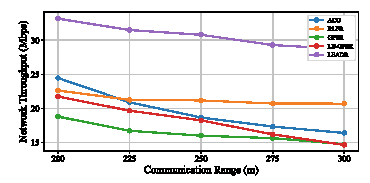
\includegraphics[width=\linewidth]{figures/rq1/com_a.pdf}
\caption{网络聚合吞吐量}\label{rq1:fig:range_a}
\end{subfigure}\hfill
\begin{subfigure}{0.49\textwidth}\centering
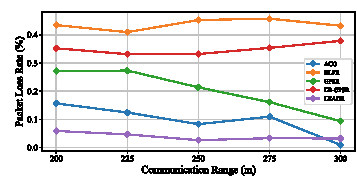
\includegraphics[width=\linewidth]{figures/rq1/com_b.pdf}
\caption{数据包丢失率}\label{rq1:fig:range_b}
\end{subfigure}
\par\medskip
\begin{subfigure}{0.49\textwidth}\centering
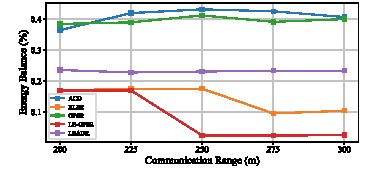
\includegraphics[width=\linewidth]{figures/rq1/com_c.pdf}
\caption{能量均衡指标}\label{rq1:fig:range_c}
\end{subfigure}\hfill
\begin{subfigure}{0.49\textwidth}\centering
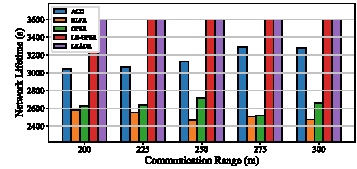
\includegraphics[width=\linewidth]{figures/rq1/com_d.pdf}
\caption{网络生命周期}\label{rq1:fig:range_d}
\end{subfigure}
\bicaption{不同通信范围下的路由性能比较}{Routing performance under different communication ranges}
\label{rq1:fig:range}
\end{figure}

图\ref{rq1:fig:range_a}中，各方法的聚合吞吐量总体随范围增加而下降，LEADR 在五个条件下均保持最高。$200\,\mathrm{m}$ 时网络通过较多中继完成转发；当范围增加至 $225\,\mathrm{m}$ 和 $250\,\mathrm{m}$，部分节点可以选择更远邻居，原有路径和竞争关系随之改变；在 $275\,\mathrm{m}$ 与 $300\,\mathrm{m}$ 条件下，LEADR 仍能维持较高的转发水平，曲线下降相对平缓。

对这一趋势需要考虑指标口径。由于聚合吞吐统计多跳转发，路径缩短会减少同一业务数据被不同节点计入的次数，因而其下降不能完全归因于最终业务送达能力恶化。另一方面，更大范围下的并发干扰和链路距离增加也会压低可达速率。图中的总体现象由这两类因素共同影响，不能只凭一条吞吐曲线分离各自贡献。相同范围条件下的方法比较仍有意义，因为各方法面对相同网络约束。

图\ref{rq1:fig:range_b}显示，LEADR 的丢包率在全部范围条件下保持较低水平，在较大通信范围下接近零。ACO 与 GPSR 的丢包率总体随范围增大而下降，说明新增邻居和较短转发路径能够缓解部分不可达问题。LB-GPSR 的曲线处于较高水平且有小幅波动，RLFR 也没有因范围扩大而获得稳定下降的丢包率。这反映出连通性改善与能量、功率管理是不同层面的因素：更多候选节点可以增加选择机会，但策略仍需有效利用这些机会。

能量离散结果如图\ref{rq1:fig:range_c}所示。LEADR 随通信范围变化保持相对平稳，低于 ACO 和 GPSR，而 LB-GPSR 在中大范围下的离散度更低，RLFR 也具有较低数值。由此可以看出，LEADR 的控制目标并不是最小化剩余能量方差本身，而是在维持服务的过程中避免过强的能量集中。其较平稳曲线表明，范围变化没有使节点能耗分布发生明显恶化；结合吞吐与丢包结果，可以认为该方法保持了较好的资源使用效率。

生命周期结果中，LEADR 与 LB-GPSR 在所有范围条件下均达到任务窗口上限，ACO、GPSR 和 RLFR 则在不同时间出现首个节点退出。扩大通信范围没有使这些基线的生命周期严格单调增长，说明拓扑可达性增强并不能替代长期能耗调节。LEADR 利用当前干扰和链路增益控制发送强度，再以邻居能量修正转发任务分配，从而在不同范围下保持完整任务周期内的通信参与能力。

\subsection{飞行速度变化下的性能分析}
\label{rq1:sec:experiment_speed}

第三组实验将平均飞行速度由 $5\,\mathrm{m/s}$ 增加至 $25\,\mathrm{m/s}$。速度变化不仅提高邻居更新频率，也会使原本持续承担中继任务的节点离开热点位置，产生新的转发机会。因而，高移动性对路由并非只有负面影响，其最终结果取决于算法能否及时利用拓扑更新。实验结果如图\ref{rq1:fig:speed}所示。

\begin{figure}[!htbp]
\centering
\begin{subfigure}{0.49\textwidth}\centering
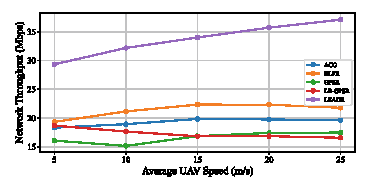
\includegraphics[width=\linewidth]{figures/rq1/speed_a.pdf}
\caption{网络聚合吞吐量}\label{rq1:fig:speed_a}
\end{subfigure}\hfill
\begin{subfigure}{0.49\textwidth}\centering
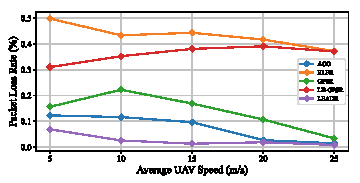
\includegraphics[width=\linewidth]{figures/rq1/speed_b.pdf}
\caption{数据包丢失率}\label{rq1:fig:speed_b}
\end{subfigure}
\par\medskip
\begin{subfigure}{0.49\textwidth}\centering
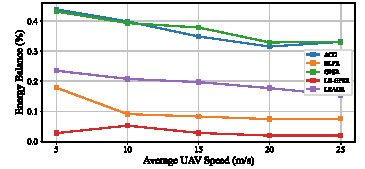
\includegraphics[width=\linewidth]{figures/rq1/speed_c.pdf}
\caption{能量均衡指标}\label{rq1:fig:speed_c}
\end{subfigure}\hfill
\begin{subfigure}{0.49\textwidth}\centering
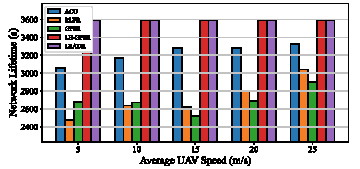
\includegraphics[width=\linewidth]{figures/rq1/speed_d.pdf}
\caption{网络生命周期}\label{rq1:fig:speed_d}
\end{subfigure}
\bicaption{不同平均飞行速度下的路由性能比较}{Routing performance at different average UAV speeds}
\label{rq1:fig:speed}
\end{figure}

图\ref{rq1:fig:speed_a}中，LEADR 的吞吐量从低速到高速条件持续上升，且始终高于对比方法。由 $5\,\mathrm{m/s}$ 增加到 $10\,\mathrm{m/s}$ 后已经出现明显增长，在 $15\,\mathrm{m/s}$、$20\,\mathrm{m/s}$ 和 $25\,\mathrm{m/s}$ 条件下继续改善。ACO 与 RLFR 的吞吐量有所提高但增幅较小，GPSR 在中间速度条件下存在波动，LB-GPSR 则总体下降。由此说明，拓扑更新带来的机会能否转化为收益，与具体转发机制密切相关。

对于轮询机制而言，按顺序轮到某一邻居时，该邻居的实际链路条件可能已经变化，原有转发顺序难以表达这种变化。LEADR 在当前邻居表上重新计算链路权重，并根据相对运动调整状态更新频率，使新出现的可用链路能够进入选择范围。与此同时，节点能量状态随实际发送过程更新，因此不会仅因某个节点暂时获得较好地理位置，就长期忽略其资源压力。

图\ref{rq1:fig:speed_b}显示，LEADR 在低速条件下已经保持较低丢包，随后随速度增加进一步下降，高速条件下接近零。ACO 与 GPSR 的丢包在部分速度条件下也有改善，说明节点移动能够打破相对固定的转发瓶颈；RLFR 和 LB-GPSR 的丢包仍保持在较高水平。该结果并不意味着飞行速度越高越好，而是说明在所设置的运动范围、通信模型和状态更新机制下，LEADR 能够利用移动带来的网络重组机会。

从图\ref{rq1:fig:speed_c}可以观察到，多个方法的能量离散度随速度增加总体下降，LEADR 同样呈下降趋势。较快移动使不同节点轮流进入有利转发位置，具有一定的自然负载分散作用。LEADR 在此基础上继续使用能量价格和下一跳能量修正，因此相较 ACO 与 GPSR 保持较小的能量差异，但其指标仍高于 LB-GPSR 和 RLFR。该结果再次表明，算法获得的是转发效率与能量分散之间的综合折中。

图\ref{rq1:fig:speed_d}中，LEADR 在五个速度条件下均达到 $3600\,\mathrm{s}$。LB-GPSR 在最低速度下未覆盖完整任务窗口，在较高速度条件下达到上限；其余基线的生命周期随速度变化呈现不同程度波动或改善。将生命周期与吞吐、丢包结合，可以看到 LEADR 在较慢运动导致转发热点持续存在时，也能够通过主动能量管理维持任务；在较快运动提供更多替代链路时，则进一步提高转发效率。

\subsection{综合讨论}

三组实验从不同角度改变网络可用资源。增加无人机数量主要改变候选中继规模和转发负载，扩大通信范围改变可达邻居、路径长度与干扰，增加飞行速度改变拓扑更新频率及热点持续时间。LEADR 在这些条件下均维持较高的聚合吞吐和较低丢包，并在观察窗口内避免通信能量耗尽造成的首个节点退出，说明将长期能量状态加入逐时隙决策具有实际作用。

同时，各指标之间存在明确取舍。LEADR 并未始终取得最小的能量离散度，部分基线也可以覆盖完整任务窗口。其主要收益在于保持持续通信能力的同时完成更多转发，并降低业务丢失。若只比较生命周期，会忽略窗口内服务量的差异；若只比较剩余能量均匀程度，又可能偏向发送活动较少的策略。因此，应以通信任务能否完成以及资源代价是否合理为判断依据。

本章实验采用给定移动模型和通信预算，对多跳转发进行系统级仿真。已展示的曲线未提供重复试验方差，因此结果分析侧重各条件下的可见趋势和指标关系，不额外给出未经统计检验的显著性判断。当前结果也未将 HELLO、接收和飞行能耗统一计入整机能源模型，后续若研究真实设备续航，应进一步扩展能耗口径。上述范围不会改变本章针对通信发射资源分配的结论，但决定了其向实际飞行任务推广时需要补充的条件。

从论文整体研究链条看，LEADR 解决的是既定数据产生后如何分配传输机会。它尚未区分不同消息对具体推理任务的价值。当无人机采集的数据量进一步增加，或上层任务只需要少量关键证据时，持续提高转发能力仍可能发送大量重复和低价值内容。因而，有必要在可用链路与能量约束之上继续研究选择性语义通信，使传输资源优先服务于能够改善协同判断的信息。

\section{本章小结}

本章针对高动态无人机网络中瞬时转发效率与长期通信能量之间的矛盾，提出能量感知分布式路由与功率联合控制策略 LEADR。通过数据队列描述服务压力，通过累计能量损耗与虚拟能量队列描述资源使用状态，推导逐时隙漂移上界，并在固定干扰的链路子问题中获得闭式功率解。在此基础上，结合下一跳剩余能量、正地理进度和自适应 HELLO 更新实现轻量分布式路由，单节点决策复杂度与邻居数量线性相关。

实验围绕无人机数量、通信范围和平均飞行速度展开，结果表明 LEADR 能够在保持较高聚合吞吐和较低丢包率的同时，使网络在设定通信预算下覆盖完整任务观察窗口。该方法通过适度的能量分散支撑更多有效转发，体现出对动态拓扑和资源约束的适应能力。下一章在此基础上把研究对象从数据转发扩展到语义证据选择，进一步分析有限通信资源应优先用于哪些消息，以提高无人机协同推理的任务收益。
